\documentclass{report}
%\usepackage[utopia]{mathdesign}
%\usepackage{amsmath, amsthm}


\usepackage{amsmath,amsfonts,amsthm,amssymb,mathtools}
\usepackage{nicefrac, xfrac}
%\usepackage[varbb]{newpxmath}
%\usepackage[osf,largesc,theoremfont]{newpxtext}
%\usepackage{coelacanth}
%\usepackage{beraserif} % Bitstream Vera Serif font
%\usepackage{berasans} % Bitstream Vera Sans font
%\usepackage{beramono} % Bitstream Vera Sans Mono font
%\usepackage{berasans}
%\usepackage{libertine}
%\usepackage{mathpazo}
%\usepackage{palatino}
%\usepackage{crimson}

% NEW ------- For pointilles lines
\usepackage{multido}

%% Choose one of the following (if not choosing the  
%% default, viz., Computer Modern, font family):
%\usepackage{lmodern}
\usepackage{bold-extra}
%%
%\usepackage{mathpazo}
% \usepackage{newpxmath}
%\usepackage{kpfonts} % Very good
%%
%\usepackage{mathptmx} %Very good
%\usepackage{stix} 
%\usepackage{txfonts} %Very good
\usepackage{newtxtext,newtxmath} %Very good
%%
%\usepackage{libertine} \usepackage[libertine]{newtxmath}
%\usepackage{libertine,libertinust1math} % added 2019/11/28
%%
%\usepackage{newpxtext} \usepackage[euler-digits]{eulervm}
%\usepackage{textcomp}
%\usepackage{bm}
\usepackage{contour}
\usepackage{adjustbox}
\usepackage{nicematrix}





\input{/home/cryptopsy/Semesters/LaTeXTemplates/UniversalTeXTemplate/preamble.tex}
%From M275 "Topology" at SJSU
\newcommand{\id}{\mathrm{id}} % Identité
\newcommand{\taking}[1]{\xrightarrow{#1}} % Flèche avec annotation
\newcommand{\inv}{^{-1}} % Inverse

%From M170 "Introduction to Graph Theory" at SJSU
\DeclareMathOperator{\diam}{diam} % Diamètre
\DeclareMathOperator{\ord}{ord} % Ordre
\newcommand{\defeq}{\overset{\mathrm{def}}{=}} % Défini comme égal

%From the USAMO .tex files
\newcommand{\ts}{\textsuperscript} % Exposant
\newcommand{\dg}{^\circ} % Degré
\newcommand{\ii}{\item} % Item

% % From Math 55 and Math 145 at Harvard
% \newenvironment{subproof}[1][Proof]{%
% \begin{proof}[#1] \renewcommand{\qedsymbol}{$\blacksquare$}}%
% {\end{proof}}

\newcommand{\liff}{\leftrightarrow} % Si et seulement si
\newcommand{\lthen}{\rightarrow} % Implique
\newcommand{\opname}{\operatorname} % Opérateur générique
\newcommand{\surjto}{\twoheadrightarrow} % Flèche surjective
\newcommand{\injto}{\hookrightarrow} % Flèche injective
\newcommand{\On}{\mathrm{On}} % Ordinaux
\DeclareMathOperator{\img}{im} % Image
\DeclareMathOperator{\Img}{Im} % Image
\DeclareMathOperator{\coker}{coker} % Cokernel
\DeclareMathOperator{\Coker}{Coker} % Cokernel
\DeclareMathOperator{\Ker}{Ker} % Noyau
\DeclareMathOperator{\rank}{rank} % Rang
\DeclareMathOperator{\Spec}{Spec} % Spectre
\DeclareMathOperator{\Tr}{Tr} % Trace
\DeclareMathOperator{\pr}{pr} % Projection
\DeclareMathOperator{\ext}{ext} % Extension
\DeclareMathOperator{\pred}{pred} % Prédécesseur
\DeclareMathOperator{\dom}{dom} % Domaine
\DeclareMathOperator{\ran}{ran} % Image (range)
\DeclareMathOperator{\Hom}{Hom} % Homomorphisme
\DeclareMathOperator{\Mor}{Mor} % Morphismes
\DeclareMathOperator{\End}{End} % Endomorphisme

\newcommand{\eps}{\epsilon} % Épsilon
\newcommand{\veps}{\varepsilon} % Variance d'épsilon
\newcommand{\ol}{\overline} % Ligne au-dessus
\newcommand{\ul}{\underline} % Ligne en-dessous
\newcommand{\wt}{\widetilde} % Tilde large
\newcommand{\wh}{\widehat} % Chapeau large
\newcommand{\vocab}[1]{\textbf{\color{blue} #1}} % Texte en gras et bleu
\providecommand{\half}{\frac{1}{2}} % Fraction 1/2
\newcommand{\dang}{\measuredangle} % Angle dirigé
\newcommand{\ray}[1]{\overrightarrow{#1}} % Ray
\newcommand{\seg}[1]{\overline{#1}} % Segment
\newcommand{\arc}[1]{\wideparen{#1}} % Arc
\DeclareMathOperator{\cis}{cis} % cis
\DeclareMathOperator*{\lcm}{lcm} % Plus petit commun multiple
\DeclareMathOperator*{\argmin}{arg min} % Argument du minimum
\DeclareMathOperator*{\argmax}{arg max} % Argument du maximum
\newcommand{\cycsum}{\sum_{\mathrm{cyc}}} % Somme cyclique
\newcommand{\symsum}{\sum_{\mathrm{sym}}} % Somme symétrique
\newcommand{\cycprod}{\prod_{\mathrm{cyc}}} % Produit cyclique
\newcommand{\symprod}{\prod_{\mathrm{sym}}} % Produit symétrique
\newcommand{\Qed}{\begin{flushright}\qed\end{flushright}} % QED aligné à droite
\newcommand{\parinn}{\setlength{\parindent}{1cm}} % Indentation de paragraphe à 1 cm
\newcommand{\parinf}{\setlength{\parindent}{0cm}} % Pas d'indentation de paragraphe
% \newcommand{\norm}{\|\cdot\|} % Norme
\newcommand{\inorm}{\norm_{\infty}} % Norme infinie
\newcommand{\opensets}{\{V_{\alpha}\}_{\alpha\in I}} % Ensemble ouvert
\newcommand{\oset}{V_{\alpha}} % Ensemble ouvert V
\newcommand{\opset}[1]{V_{\alpha_{#1}}} % Ensemble ouvert V avec indice
\newcommand{\lub}{\text{lub}} % Plus petite borne supérieure
\newcommand{\del}[2]{\frac{\partial #1}{\partial #2}} % Dérivée partielle
\newcommand{\Del}[3]{\frac{\partial^{#1} #2}{\partial^{#1} #3}} % Dérivée partielle d'ordre élevé
\newcommand{\deld}[2]{\dfrac{\partial #1}{\partial #2}} % Dérivée partielle avec dfrac
\newcommand{\Deld}[3]{\dfrac{\partial^{#1} #2}{\partial^{#1} #3}} % Dérivée partielle d'ordre élevé avec dfrac
\newcommand{\lm}{\lambda} % Lambda
\newcommand{\uin}{\mathbin{\rotatebox[origin=c]{90}{$\in$}}} % Appartient, tourné de 90 degrés
\newcommand{\usubset}{\mathbin{\rotatebox[origin=c]{90}{$\subset$}}} % Sous-ensemble, tourné de 90 degrés
\newcommand{\lt}{\left} % Gauche
\newcommand{\rt}{\right} % Droite
\newcommand{\bs}[1]{\boldsymbol{#1}} % Symbole en gras
\newcommand{\exs}{\exists} % Il existe
\newcommand{\st}{\strut} % Strut
\newcommand{\dps}[1]{\displaystyle{#1}} % Disposition en ligne

\newcommand{\sol}{\setlength{\parindent}{0cm}\textbf{\textit{Solution:}}\setlength{\parindent}{1cm} } % Solution sans indentation initiale puis rétablie
\newcommand{\solve}[1]{\setlength{\parindent}{0cm}\textbf{\textit{Solution: }}\setlength{\parindent}{1cm}#1 \Qed}

\newcommand{\entoure}[1]{\fcolorbox{black}{gray!30}{\texttt{#1}}}

\renewcommand{\ttdefault}{cmtt}
\newcommand{\textttbf}[1]{\contour{yellow!45}{\texttt{#1}}}
\newcommand{\varitem}[3][black]{%
    \item [%
        \colorbox{#2}{\textcolor{#1}{\makebox(5.5,7){#3}}}%
    ]
}
% Allow you to do the non implication (implication barred)
\newcommand{\notimplies}{%
  \mathrel{{\ooalign{\hidewidth$\not\phantom{=}$\hidewidth\cr$\implies$}}}}


\newcommand*{\authorimg}[1]%
    { \raisebox{-1\baselineskip}{\includegraphics[width=\imagesize]{#1}}}
\newlength\imagesize 

\input{/home/cryptopsy/Semesters/LaTeXTemplates/UniversalTeXTemplate/letterfonts.tex}
% lstlistingsEnvs.tex

\usepackage{minted}


\lstset{
  basicstyle=\ttfamily, % Set
  columns=fullflexible,
  keepspaces=true,
  language=Python % You can specify the language if you want syntax highlighting
}

%%%%%%%%%%%%%%%%%%%%%%%%%%%%%%%%%%%%%%%%%%%%%%%%%%%%%%%%%%%%%%%%%%%%%%%%%%%%%%%%%%%%%%%%%%%%%%%%%
%                                 Custom lstlisting Environments
%%%%%%%%%%%%%%%%%%%%%%%%%%%%%%%%%%%%%%%%%%%%%%%%%%%%%%%%%%%%%%%%%%%%%%%%%%%%%%%%%%%%%%%%%%%%%%%%%
% Gruvbox style for Python
\definecolor{Pgruvbox-bg}{HTML}{282828}
\definecolor{Pgruvbox-fg}{HTML}{ebdbb2}
\definecolor{Pgruvbox-red}{HTML}{fb4934}
\definecolor{Pgruvbox-green}{HTML}{b8bb26}
\definecolor{Pgruvbox-yellow}{HTML}{fabd2f}
\definecolor{Pgruvbox-blue}{HTML}{83a598}
\definecolor{Pgruvbox-purple}{HTML}{d3869b}
\definecolor{Pgruvbox-aqua}{HTML}{8ec07c}
\definecolor{BBBlack}{rgb}{0.05, 0.06, 0.09}



% JAVA LSTLISTING STYLE IN Gruvbox Colorscheme
\definecolor{gruvbox-bg}{rgb}{0.282, 0.247, 0.204}
\definecolor{gruvbox-fg1}{rgb}{0.949, 0.898, 0.776}
\definecolor{gruvbox-fg2}{rgb}{0.871, 0.804, 0.671}
\definecolor{gruvbox-red}{rgb}{0.788, 0.255, 0.259}
\definecolor{gruvbox-green}{rgb}{0.518, 0.604, 0.239}
\definecolor{gruvbox-yellow}{rgb}{0.914, 0.808, 0.427}
\definecolor{gruvbox-blue}{rgb}{0.353, 0.510, 0.784}
\definecolor{gruvbox-purple}{rgb}{0.576, 0.412, 0.659}
\definecolor{gruvbox-aqua}{rgb}{0.459, 0.631, 0.737}
\definecolor{gruvbox-gray}{rgb}{0.518, 0.494, 0.471}

\definecolor{lst-bg}{RGB}{45, 45, 45}
\definecolor{lst-fg}{RGB}{220, 220, 204}
\definecolor{lst-keyword}{RGB}{215, 186, 125}
\definecolor{lst-comment}{RGB}{117, 113, 94}
\definecolor{lst-string}{RGB}{163, 190, 140}
\definecolor{lst-number}{RGB}{181, 206, 168}
\definecolor{lst-type}{RGB}{218, 142, 130}

\lstdefinestyle{PythonGruvbox}{
    language=Python,
    identifierstyle=\color{lst-fg},
    basicstyle=\ttfamily\color{Pgruvbox-fg},
    keywordstyle=\color{Pgruvbox-yellow},
    keywordstyle=[2]\color{Pgruvbox-blue},
    stringstyle=\color{Pgruvbox-green},
    commentstyle=\color{Pgruvbox-aqua},
    backgroundcolor=\color{BBBlack},
    rulecolor=\color{BBBlack},
    showstringspaces=false,
    keepspaces=true,
    captionpos=b,
    breaklines=true,
    tabsize=4,
    showspaces=false,
    numbers=left,
    numbersep=5pt,
    numberstyle=\tiny\color{gray},
    showtabs=false,
    columns=fullflexible,
    morekeywords={True,False,None},
    morekeywords=[2]{and,as,assert,break,class,continue,def,del,elif,else,except,exec,
    finally,for,from,global,if,import,in,is,lambda,nonlocal,not,or,pass,print,raise,
    return,try,while,with,yield},
    morecomment=[s]{"""}{"""},
    morecomment=[s]{'''}{'''},
    morecomment=[l]{\#},
    morestring=[b]",
    morestring=[b]',
    literate=
    {0}{{\textcolor{Pgruvbox-purple}{0}}}{1}
    {1}{{\textcolor{Pgruvbox-purple}{1}}}{1}
    {2}{{\textcolor{Pgruvbox-purple}{2}}}{1}
    {3}{{\textcolor{Pgruvbox-purple}{3}}}{1}
    {4}{{\textcolor{Pgruvbox-purple}{4}}}{1}
    {5}{{\textcolor{Pgruvbox-purple}{5}}}{1}
    {6}{{\textcolor{Pgruvbox-purple}{6}}}{1}
    {7}{{\textcolor{Pgruvbox-purple}{7}}}{1}
    {8}{{\textcolor{Pgruvbox-purple}{8}}}{1}
    {9}{{\textcolor{Pgruvbox-purple}{9}}}{1}
}

% Gruvbox style for Java
\definecolor{gruvbox-bg}{rgb}{0.282, 0.247, 0.204}
\definecolor{gruvbox-fg1}{rgb}{0.949, 0.898, 0.776}
\definecolor{gruvbox-fg2}{rgb}{0.871, 0.804, 0.671}
\definecolor{gruvbox-red}{rgb}{0.788, 0.255, 0.259}
\definecolor{gruvbox-green}{rgb}{0.518, 0.604, 0.239}
\definecolor{gruvbox-yellow}{rgb}{0.914, 0.808, 0.427}
\definecolor{gruvbox-blue}{rgb}{0.353, 0.510, 0.784}
\definecolor{gruvbox-purple}{rgb}{0.576, 0.412, 0.659}
\definecolor{gruvbox-aqua}{rgb}{0.459, 0.631, 0.737}
\definecolor{gruvbox-gray}{rgb}{0.518, 0.494, 0.471}

\lstdefinestyle{JavaGruvbox}{
    language=Java,
    basicstyle=\ttfamily\color{Pgruvbox-fg},
    keywordstyle=\color{Pgruvbox-yellow},
    keywordstyle=[2]\color{lst-type},
    commentstyle=\itshape\color{lst-comment},
    stringstyle=\color{lst-string},
    numberstyle=\color{lst-number},
    backgroundcolor=\color{BBBlack},
    rulecolor=\color{gruvbox-aqua},
    showstringspaces=false,
    keepspaces=true,
    captionpos=b,
    breaklines=true,
    tabsize=4,
    showspaces=false,
    showtabs=false,
    columns=fullflexible,
    morekeywords={var},
    morekeywords=[2]{boolean, byte, char, double, float, int, long, short, void},
    morecomment=[s]{/}{/},
    morecomment=[l]{//},
    morestring=[b]",
    morestring=[b]',
    numbers=left,
    numbersep=5pt,
    numberstyle=\tiny\color{gray},
}

% Dracula style for Java
\definecolor{draculawhite-background}{RGB}{237, 239, 252}
\definecolor{draculawhite-comment}{RGB}{98, 114, 164}
\definecolor{draculawhite-keyword}{RGB}{189, 147, 249}
\definecolor{draculawhite-string}{RGB}{152, 195, 121}
\definecolor{draculawhite-number}{RGB}{249, 189, 89}
\definecolor{draculawhite-operator}{RGB}{248, 248, 242}

\lstdefinestyle{JavaDraculaWhite}{
    language=Java,
    backgroundcolor=\color{draculawhite-background},
    commentstyle=\itshape\color{draculawhite-comment},
    keywordstyle=\color{draculawhite-keyword},
    stringstyle=\color{draculawhite-string},
    basicstyle=\ttfamily\footnotesize\color{black},
    identifierstyle=\color{black},
    keywordstyle=\color{draculawhite-keyword}\bfseries,
    morecomment=[s][\color{draculawhite-comment}]{/**}{*/},
    showstringspaces=false,
    showspaces=false,
    breaklines=true,
    %frame=single,
    rulecolor=\color{draculawhite-operator},
    tabsize=2,  
    numbers=left,
    numbersep=4pt,
    numberstyle=\ttfamily\tiny\color{gray}
}

% Dracula style for Python
\definecolor{draculawhite-bg}{HTML}{FAFAFA}
\definecolor{draculawhite-fg}{HTML}{282A36}
\definecolor{pdraculawhite-keyword}{HTML}{BD93F9}
\definecolor{pdraculawhite-comment}{HTML}{6272A4}
\definecolor{draculawhite-number}{HTML}{FF79C6}

\lstdefinestyle{PythonDraculaWhite}{
    language=Python,
    basicstyle=\ttfamily\small\color{draculawhite-fg},
    backgroundcolor=\color{draculawhite-background},
    keywordstyle=\color{orange}\bfseries,
    stringstyle=\color{draculawhite-string},
    commentstyle=\color{pdraculawhite-comment}\itshape,
    numberstyle=\color{draculawhite-number},
    showstringspaces=false,
    showspaces=false,
    breaklines=true,
    frame=single,
    rulecolor=\color{draculawhite-operator}, 
    tabsize=4,
    morekeywords={as,with,1,2,3,4, 5,6,7,8,9,True,False},
    numbers=left,
    numbersep=5pt,
    numberstyle=\small\bfseries\ttfamily\color{htmlcomment},
}

% Dracula Dark style for HTML
\definecolor{htmltag}{HTML}{ff79c6}
\definecolor{htmlattr}{HTML}{f1fa8c}
\definecolor{htmlvalue}{HTML}{bd93f9}
\definecolor{htmlcomment}{HTML}{6272a4}
\definecolor{htmltext}{HTML}{401E31}
\definecolor{htmlbackground}{HTML}{282a36}
\definecolor{comphtmlbackground}{HTML}{8093FF}

\lstdefinestyle{HTMLDraculaDark}{
    basicstyle=\normalsize\bfseries\ttfamily\color{htmltext},
    commentstyle=\itshape\color{htmlcomment},
    keywordstyle=\bfseries\color{htmltag},
    stringstyle=\color{htmlvalue},
    emph={DOCTYPE,html,head,body,div,span,a,script},
    emphstyle={\color{htmltag}\bfseries},
    sensitive=true,
    showstringspaces=false,
    backgroundcolor=\color{white},
    inputencoding=utf8,
    extendedchars=true,
    language=HTML,
    tabsize=4,
    breaklines=true,
    breakatwhitespace=true,
    numbers=left,
    numbersep=10pt,
    numberstyle=\small\bfseries\ttfamily\color{htmlcomment},
    escapeinside={<@}{@>},
    rulecolor=\color{htmlbackground},
    xleftmargin=10pt,
    frame=none, 
    breaklines=true,
    postbreak=\mbox{\textcolor{gray}{$\hookrightarrow$}\space},
    showlines=false,
    moredelim=[s][\itshape\color{htmlcomment}]{<!--}{-->},
    morekeywords={id,class,type,name,value,placeholder,checked,src,href,alt},
    literate={é}{{\'e}}1 {è}{{\`e}}1 {ê}{{\^e}}1 {ë}{{\"e}}1 {à}{{\`a}}1 {ù}{{\`u}}1 {û}{{\^u}}1 {ç}{{\c{c}}}1 {â}{{\^a}}1 {î}{{\^i}}1 {ï}{{\"i}}1
}


\lstdefinestyle{Haskell}{
  frame=none,
  xleftmargin=2pt,
  stepnumber=1,
  numbers=left,
  numbersep=5pt,
  numberstyle=\ttfamily\tiny\color[gray]{0.3},
  belowcaptionskip=\bigskipamount,
  captionpos=b,
  escapeinside={*'}{'*},
  language=haskell,
  tabsize=2,
  emphstyle={\bf},
  %commentstyle=\it,
  stringstyle=\mdseries\ttfamily,
  showspaces=false,
  keywordstyle=\bfseries\ttfamily,
  columns=flexible,
  basicstyle=\small\ttfamily,
  showstringspaces=false,
  morecomment=[l]\%,
}



\lstdefinestyle{CSSDraculaLight}{
    basicstyle=\bfseries\scriptsize\ttfamily\color{htmltext},
    commentstyle=\color{htmlcomment},
    keywordstyle=\bfseries\color{htmlvalue},
    stringstyle=\color{htmlvalue},
    emph={DOCTYPE,html,head,body,div,span,a,script},
    emphstyle={\color{htmltag}\bfseries},
    sensitive=true,
    showstringspaces=false,
    backgroundcolor=\color{white},
    inputencoding=utf8,
    extendedchars=true, % Support extended characters
    frame=none, 
    %frame=tb,
    tabsize=4,
    breaklines=true,
    breakatwhitespace=true,
    numbers=left,
    numbersep=10pt,
    numberstyle=\small\bfseries\ttfamily\color{htmlcomment},
    escapeinside={<@}{@>},
    rulecolor=\color{htmlbackground},
    xleftmargin=20pt,
    % Add a vertical line for opening and closing tags
    %frame=lines,
    framesep=2pt,
    framexleftmargin=4pt,
    % Add a vertical line for closing tags that go through multiple lines
    breaklines=true,
    postbreak=\mbox{\textcolor{gray}{$\hookrightarrow$}\space},
    showlines=true,
    % Add a rule to apply commentstyle to keywords inside comments
    moredelim=[s][\color{htmlcomment}]{/*}{*/},
    literate={é}{{\'e}}1
             {è}{{\`e}}1
             {ê}{{\^e}}1
             {ë}{{\"e}}1
             {à}{{\`a}}1
             {ù}{{\`u}}1
             {û}{{\^u}}1
             {ç}{{\c{c}}}1
             {â}{{\^a}}1
             {î}{{\^i}}1
             {ï}{{\"i}}1,
    morekeywords={color, background, background-color, font-size, font-weight, border, border-radius, padding, margin, display, position, top, right, bottom, left, flex, grid, width, height, min-width, max-width, min-height, max-height, transition, transform, animation, keyframes, content, z-index,id,class,type,name,value,placeholder,checked,src,href,alt},
    morestring=[s][\color{htmltag}]{:}{;},
}










\title{\huge{IFT-1575}\\\Huge{Modèles de recherche opérationnelle}\\\vspace{2em} Introduction}
\author{\huge{Franz Girardin}}
\date{\today}


% NEW for point lines
\newcommand{\Pointilles}[1]{%
  \par\nobreak
  \noindent\rule{0pt}{1.5\baselineskip}% Provides a larger gap between the preceding paragraph and the dots
  \multido{}{#1}{\noindent\makebox[\linewidth]{\dotfill}\endgraf}% ... dotted lines ...
  \bigskip% Gap between dots and next paragraph
}
% Define a new command for dotted lines that works in align
\newcommand{\PointillesAlign}{%
  \multido{}{1}{\makebox[\linewidth]{\dotfill}}
}

   

\begin{document}
\begin{multicols*}{2}
\chapter{Algorithme du Simplexe}
\section{Forme algébrique de l'algorithme}
\begin{itemize}
    \item[$\blacktriangleright$] \textbf{Forme standard} :
    \begin{align*}
        \text{Minimiser } & z = c_1x_1 + c_2x_2 + \dots + c_nx_n \\
        \text{s.a. } &
        \begin{cases}
            a_{11}x_1 + a_{12}x_2 + \dots + a_{1n}x_n \leq b_1 \\
            \vdots \\
            a_{m1}x_1 + a_{m2}x_2 + \dots + a_{mn}x_n \leq b_m \\
            x_1, x_2, \dots, x_n \geq 0
        \end{cases}
    \end{align*}

    \item[$\blacktriangleright$] \textbf{Introduction des variables d'écart} $s_i$ :
    \[
    a_{i1}x_1 + a_{i2}x_2 + \dots + a_{in}x_n + s_i = b_i, \quad s_i \geq 0
    \]

    \item[$\blacktriangleright$] \textbf{Fonction objectif ajustée} :
    \[
    z + c_1x_1 + c_2x_2 + \dots + c_nx_n = 0
    \]

    \item[$\blacktriangleright$] \textbf{Choix de la variable entrante} :
    \begin{itemize}
        \item[$\rhd$] Sélectionner la variable avec le coefficient \textbf{le plus négatif} dans la fonction objectif.
    \end{itemize}

    \item[$\blacktriangleright$] \textbf{Détermination de la variable sortante} :
    \begin{itemize}
        \item[$\rhd$] Calculer le \textbf{ratio} pour chaque contrainte :
        \[
        \boxed{\text{Ratio} = \dfrac{b_i}{a_{ij}}} \quad \text{avec } a_{ij} > 0
        \]
        \item[$\rhd$] La variable avec le plus petit ratio positif est la \textbf{variable sortante}.
        \item[$\rhd$] Si tous les $a_{ij}$ sont négatifs, on conclue 
            alors que le problème est \textbf{non borné}                        .
    \end{itemize}

    \item[$\blacktriangleright$] \textbf{Pivot} :
    \begin{itemize}
        \item[$\rhd$] Mettre à jour le tableau en pivotant sur le coefficient correspondant.
    \end{itemize}

    \item[$\blacktriangleright$] \textbf{Critère d'optimalité} :
    \begin{itemize}
        \item[$\rhd$] Si tous les coefficients $\overline{c}_j$de la fonction objectif sont tels que 
            $\overline{c}_j \geq 0$, la solution est optimale.
    \end{itemize}

    \item[$\blacktriangleright$] \textbf{Formules importantes} :
    \begin{itemize}
        \item[$\rhd$] \textbf{Coefficient réduit} :
        \[
        \boxed{\overline{c}_j = c_j - \sum_{i} c_i^{B} a_{ij}}
        \]
        \item[$\rhd$] \textbf{Mise à jour des coefficients} :
        \begin{align*}
            & \text{Nouvelle ligne pivot} : 
         \\ &\quad \hspace{-2em}\boxed{\text{Ligne pivot} \div \text{Coefficient pivot}} \\
            & \text{Autres lignes} : 
         \\ &\hspace{-4em}\boxed{\text{Ligne} - (\text{Coefficient} \times \text{Nouvelle ligne pivot})}
        \end{align*}
    \end{itemize}

    \item[$\blacktriangleright$] \textbf{Résumé des étapes} :
    \begin{enumerate}
        \item[$\rhd$] Formuler le problème en forme standard.
        \item[$\rhd$] Identifier la variable entrante (coefficient le plus négatif).
        \item[$\rhd$] Trouver la variable sortante (plus petit ratio positif).
        \item[$\rhd$] Effectuer le pivot.
        \item[$\rhd$] Répéter jusqu'à optimalité.
    \end{enumerate}
\end{itemize}

\section{Forme Tabulée de l'algorithme}
\begin{itemize}
    \item[$\blacktriangleright$] \textbf{Construction du Tableau Simplexe} :
    \begin{itemize}
        \item[$\rhd$] Organiser les équations du problème en \textbf{forme standard} dans un tableau.
        \item[$\rhd$] La première colonne contient les \textbf{variables de base} (variables dépendantes).
        \item[$\rhd$] Chaque ligne représente une équation, y compris la fonction objectif négative $(-z)$.
    \end{itemize}
    
    \item[$\blacktriangleright$] \textbf{Choix de la Variable Entrante} :
    \begin{itemize}
        \item[$\rhd$] Sélectionner la variable avec le coefficient le plus négatif dans la ligne $(-z)$.
        \item[$\rhd$] Cette variable améliorera le plus la valeur de l'objectif.
    \end{itemize}
    
    \item[$\blacktriangleright$] \textbf{Détermination de la Variable Sortante} :
    \begin{itemize}
        \item[$\rhd$] Calculer les \textbf{ratios} pour chaque variable de base :
        \[
        \boxed{\text{Ratio} = \dfrac{\text{Terme de droite}}{\text{Coefficient de la variable entrante}}}
        \]
        \item[$\rhd$] Ignorer les coefficients négatifs ou nuls de la variable entrante.
        \item[$\rhd$] La variable avec le plus petit ratio positif est la \textbf{variable sortante}.
    \end{itemize}
    
    \item[$\blacktriangleright$] \textbf{Pivot} :
    \begin{itemize}
        \item[$\rhd$] Identifier le \textbf{coefficient pivot} à l'intersection de la colonne de la variable entrante et de la ligne de la variable sortante.
        \item[$\rhd$] Diviser la ligne pivot par le coefficient pivot pour obtenir un 1.
        \item[$\rhd$] Utiliser des opérations sur les lignes pour annuler les autres coefficients dans la colonne de la variable entrante.
    \end{itemize}
    
    \item[$\blacktriangleright$] \textbf{Itération} :
    \begin{itemize}
        \item[$\rhd$] Répéter le processus de sélection des variables entrante et sortante, suivi du pivot, jusqu'à ce que tous les coefficients de $(-z)$ soient positifs ou nuls.
    \end{itemize}
    
    \item[$\blacktriangleright$] \textbf{Solution Optimale} :
    \begin{itemize}
        \item[$\rhd$] Lorsque tous les coefficients de $(-z)$ sont positifs ou nuls, la solution optimale est atteinte.
        \item[$\rhd$] Les valeurs des variables de base se trouvent dans la colonne des termes de droite.
    \end{itemize}
    
    \item[$\blacktriangleright$] \textbf{Nombre de Solutions de Base} :
\hspace{-4em}
    \begin{itemize}
        \item[$\rhd$] Pour un système avec $n$ variables et $m$ équations :
        \[
            \hspace{-2em}\boxed{\text{Nombre de solutions de base} = {n \choose m} = \dfrac{n!}{m!(n-m)!}}
        \]
    \end{itemize}
    
    \item[$\blacktriangleright$] \textbf{Résumé des Étapes} :
    \begin{enumerate}
        \item[$\rhd$] \textbf{Organiser} les équations en tableau.
        \item[$\rhd$] \textbf{Choisir} la variable entrante ($x_s$) avec le coefficient le plus négatif dans $(-z)$.
        \item[$\rhd$] \textbf{Déterminer} la variable sortante ($x_r$) avec le plus petit ratio positif.
        \item[$\rhd$] \textbf{Effectuer} le pivot sur le coefficient pivot.
        \item[$\rhd$] \textbf{Répéter} jusqu'à optimalité.
    \end{enumerate}
\end{itemize}

\section{Résolution Graphique}

\begin{itemize}
    \item[$\blacktriangleright$] \textbf{Méthode de Résolution Graphique} (pour problèmes à deux variables) :
    \begin{enumerate}
        \item[$\rhd$] \textbf{Tracer les contraintes} sur un plan cartésien :
        \begin{itemize}
            \item[$\rhd$] Convertir chaque inégalité en équation pour tracer la droite correspondante.
            \item[$\rhd$] Identifier la zone admissible (région des solutions réalisables) en tenant compte des inégalités.
        \end{itemize}
        \item[$\rhd$] \textbf{Déterminer les sommets} de la zone admissible :
        \begin{itemize}
            \item[$\rhd$] Trouver les points d'intersection des droites (sommets du polygone formé).
        \end{itemize}
        \item[$\rhd$] \textbf{Calculer la valeur de la fonction objectif} en chaque sommet :
        \begin{itemize}
            \item[$\rhd$] Évaluer $z = c_1x + c_2y$ pour chaque couple $(x, y)$.
        \end{itemize}
        \item[$\rhd$] \textbf{Choisir la solution optimale} :
        \begin{itemize}
            \item[$\rhd$] Pour une maximisation, sélectionner le sommet avec la valeur de $z$ la plus élevée.
            \item[$\rhd$] Pour une minimisation, choisir le sommet avec la valeur de $z$ la plus faible.
        \end{itemize}
    \end{enumerate}
\end{itemize}

\begin{center}
\begin{tikzpicture}[scale=0.35]
    % Axe des x et des y
    \draw[->] (-1,0) -- (18,0) node[right] {$x$};
    \draw[->] (0,-1) -- (0,12.5) node[above] {$y$};
    
    % Tracer la droite 5x + 3y = 30 en rouge
    \draw[red, thick] (0,10) -- (6,0) 
     node at (3, 11) {$5x + 3y = 30$};
        
    % Tracer la droite x + 3y = 18
    \draw[myg, thick] (0,18/3) -- (18,0) 
     node at (6.5, 6) {$x + 3y = 18$};



    % Tracer la droite 2x + 3y = 24 en bleu
    \draw[blue, thick] (0,8) -- (12,0) 
    node at (4.5,8.5) {$2x + 3y = 24$};
    
    
    % Hachures pour la région de la solution
    \fill[red!20,opacity=0.6] (0,10) -- (6,0) -- (0,0) -- cycle;
    \fill[blue!20,opacity=0.6] (0,8) -- (12,0) -- (0,0) -- cycle;
    \fill[myg!20,opacity=0.6] (0,18/3) -- (18,0) -- (0,0) -- cycle;


 % Tracer les lignes d'intersection plus épaisses
    \draw[myp!70!blue, ultra thick] (0,6) -- (3,5); % Intersection rouge-bleu
    \draw[myp!70!blue, ultra thick] (3,5) -- (6,0); % Intersection rouge-bleu
    \draw[myp!70!blue, ultra thick] (6,0) -- (0,0); % Intersection rouge-bleu
    \draw[myp!70!blue, ultra thick] (0,0) -- (0,6); % Intersection rouge-bleu

    % Hachures pour la région de solution commune, avec une couleur plus foncée
    \fill[red!50!blue!50!myg!50, opacity=0.8] (0,6) -- (3,5) -- (6,0) -- (0,0) -- cycle;
    
    % Ajouter des labels
\end{tikzpicture}
\end{center}

\subsection*{Notes Importantes}
\begin{itemize}
    \item[$\blacktriangleright$] \textbf{Dans un problème à deux variables}, la zone admissible est un polygone convexe sur le plan $xy$, et la solution optimale se trouve toujours à l'un des sommets de ce polygone.

    \item[$\blacktriangleright$] \textbf{Vérification de la Faisabilité} :
    \begin{itemize}
        \item[$\rhd$] S'assurer que les points trouvés respectent toutes les contraintes.
    \end{itemize}

    \item[$\blacktriangleright$] \textbf{Cas Particuliers} :
    \begin{itemize}
        \item[$\rhd$] \textbf{Solutions Multiples} : Si la fonction objectif est parallèle à une contrainte bordant la région admissible.
        \item[$\rhd$] \textbf{Région Non Bornée} : Si la région admissible n'est pas limitée, la solution optimale peut être non bornée.
    \end{itemize}
\end{itemize}


\section{Forme Générale de l'Algorithme}

    \begin{itemize}
        \item[$\blacktriangleright$] \textbf{Notations} :
            \begin{itemize}
                \item[$\rhd$] \( x_j \) : Variables de décision, \( j = 1, 2, \dots, n \).
                \item[$\rhd$] \( c_j \) : Coefficients dans la fonction objectif.
                \item[$\rhd$] \( a_{ij} \) : Coefficients des contraintes, \( i = 1, 2, \dots, m \).
                \item[$\rhd$] \( b_i \) : Termes de droite des contraintes.
            \end{itemize}

        \item[$\blacktriangleright$] \textbf{Forme Standard} :
        \[%
            \begin{aligned}
            \text{Minimiser } & z = \sum_{j=1}^{n} c_j x_j \\
            \text{sous contraintes } & \sum_{j=1}^{n} a_{ij} x_j = b_i, \quad i = 1, 2, \dots, m \\
            & x_j \geq 0, \quad j = 1, 2, \dots, n
            \end{aligned}
        \]%

        \item[$\blacktriangleright$] \textbf{Tableau Simplexe Général} :
            \begin{itemize}
                \item[$\rhd$] Les variables de base \( x_i \) forment une base identité.
                \item[$\rhd$] Les variables non de base sont initialement fixées à zéro.
            \end{itemize}

        \item[$\blacktriangleright$] \textbf{Choix de la Variable Entrante} :
            \begin{itemize}
                \item[$\rhd$] Si tous les coefficients réduits \( \overline{c}_j \geq 0 \), la solution est optimale.
                \item[$\rhd$] Sinon, choisir \( x_s \) tel que :
                \[%
                \boxed{\overline{c}_s = \min \{ c_j \mid j = 1, 2, \dots, n \}}
                \]%
            \end{itemize}

        \item[$\blacktriangleright$] \textbf{Détermination de la Variable Sortante} :
            \begin{itemize}
                \item[$\rhd$] Calculer les ratios pour \( \overline{a}_{is} > 0 \) :
                \[%
                \boxed{\text{Ratio} = \dfrac{\overline{b}_i}{\overline{a}_{is}}}
                \]%
                \item[$\rhd$] La variable sortante \( x_r \) correspond au plus petit ratio positif.
                \item[$\rhd$] Si \( \overline{a}_{is} \leq 0 \) pour tout \( i \), le problème est non borné.
            \end{itemize}

        \item[$\blacktriangleright$] \textbf{Pivot et Mise à Jour du Tableau} :
        \begin{itemize}
            \item[$\rhd$] \textbf{Ligne Pivot} (\( r \)) :
            \[
            \boxed{\text{Nouvelle ligne } r = \dfrac{\text{Ancienne ligne } r}{\overline{a}_{rs}}}
            \]
            \item[$\rhd$] \textbf{Autres Lignes} (\( i \neq r \)) :
            \[
                \hspace{-4em}\boxed{\text{Nouvelle ligne } i = \text{Ancienne ligne } i - \overline{a}_{is} \times \text{Nouvelle ligne } r}
            \]
            \item[$\rhd$] \textbf{Fonction Objectif} :
            \[
                \boxed{\overline{\tilde{c}}_j = \overline{c}_j - \overline{c}_s \times \overline{a}_{rj}}
            \]
            \[
                \boxed{\overline{\tilde{z}} = \overline{z} + \overline{c}_s \times \overline{b}_r}
            \]
        \end{itemize}

    \item[$\blacktriangleright$] \textbf{Résumé des Étapes de l'Algorithme} :
    \begin{enumerate}
        \item[$\rhd$] \textbf{Initialisation} : Formuler le problème en forme standard et construire le tableau initial.
        \item[$\rhd$] \textbf{Itération} :
        \begin{enumerate}
            \item[$\rhd$] Choisir la variable entrante \( x_s \) avec le \( \overline{c}_s \) le plus négatif.
            \item[$\rhd$] Déterminer la variable sortante \( x_r \) en calculant les ratios.
            \item[$\rhd$] Effectuer le pivot pour mettre à jour le tableau.
        \end{enumerate}
        \item[$\rhd$] \textbf{Vérification d'Optimalité} :
        \begin{itemize}
            \item[$\rhd$] Si tous les \( \overline{c}_j \geq 0 \), la solution optimale est atteinte.
            \item[$\rhd$] Sinon, répéter l'itération.
        \end{itemize}
    \end{enumerate}

    \item[$\blacktriangleright$] \textbf{Formules Clés} :
    \begin{itemize}
        \item[$\rhd$] \textbf{Mise à Jour des Coefficients} :
        \[
            \boxed{\overline{\tilde{a}}_{ij} = \overline{a}_{ij} - \overline{a}_{is} \times \overline{a}_{rj}}
        \]
        \item[$\rhd$] \textbf{Mise à Jour des Termes de Droite} :
        \[
            \boxed{\overline{\tilde{b}}_i = \overline{b}_i - \overline{a}_{is} \times \overline{b}_r}
        \]
    \end{itemize}
\end{itemize}
\section{Forme Matricielle de l'Algorithme}

\subsection*{Notations Matricielles}

\begin{itemize}
    \item[$\blacktriangleright$] \textbf{Variables de Décision} :
    \[
    \mathbf{x}_{n \times 1} = 
    \begin{bmatrix}
    x_1 \\
    x_2 \\
    \vdots \\
    x_n
    \end{bmatrix}
    \]
    \item[$\blacktriangleright$] \textbf{Coefficients de l'Objectif} :
    \[
    \mathbf{c}_{n \times 1} = 
    \begin{bmatrix}
    c_1 \\
    c_2 \\
    \vdots \\
    c_n
    \end{bmatrix}
    \]
    \item[$\blacktriangleright$] \textbf{Matrice des Contraintes} :
    \[
    \mathbf{A}_{m \times n} = 
    \begin{bmatrix}
    a_{11} & a_{12} & \cdots & a_{1n} \\
    a_{21} & a_{22} & \cdots & a_{2n} \\
    \vdots & \vdots & \ddots & \vdots \\
    a_{m1} & a_{m2} & \cdots & a_{mn}
    \end{bmatrix}
    \]
    \item[$\blacktriangleright$] \textbf{Termes de Droite} :
    \[
    \mathbf{b}_{m \times 1} = 
    \begin{bmatrix}
    b_1 \\
    b_2 \\
    \vdots \\
    b_m
    \end{bmatrix}
    \]
\end{itemize}

\subsection*{Formulation Matricielle du Problème}

Le problème de programmation linéaire en forme standard peut être écrit en notation matricielle comme suit :

\begin{align*}
& \text{Minimiser} \quad z = \mathbf{c}^T \mathbf{x} \\
& \text{sous contraintes} \quad \mathbf{A} \mathbf{x} = \mathbf{b} \\
& \quad \quad \quad \quad \quad \mathbf{x} \geq 0
\end{align*}

\subsection*{Interprétation}

\begin{itemize}
    \item[$\rhd$] \textbf{Objectif} : \(\mathbf{c}^T \mathbf{x} = \sum_{j=1}^{n} c_j x_j\)
    \item[$\rhd$] \textbf{Contraintes} : Chaque équation \( \sum_{j=1}^{n} a_{ij} x_j = b_i \) est représentée par le produit matriciel \( \mathbf{A} \mathbf{x} = \mathbf{b} \)
    \item[$\rhd$] \textbf{Non-négativité} : \( \mathbf{x} \geq 0 \) signifie que chaque \( x_j \geq 0 \)
\end{itemize}

\subsection*{Exemple : Problème du Restaurateur}

Considérons le problème du restaurateur avec les variables \( x \) et \( y \), et les variables d'écart \( u, p, h \).

\begin{align*}
& \text{Minimiser} \quad z = 8x + 6y \\
& \text{sous contraintes} \\
& 5x + 3y + u = 30 \\
& 2x + 3y + p = 24 \\
& x + 3y + h = 18 \\
& x, y, u, p, h \geq 0
\end{align*}

En notation matricielle :

\[
\mathbf{x} = 
\begin{bmatrix}
x \\ y \\ u \\ p \\ h
\end{bmatrix}, \quad
\mathbf{c} = 
\begin{bmatrix}
-8 \\ -6 \\ 0 \\ 0 \\ 0
\end{bmatrix}, \quad
\mathbf{A} = 
\begin{bmatrix}
5 & 3 & 1 & 0 & 0 \\
2 & 3 & 0 & 1 & 0 \\
1 & 3 & 0 & 0 & 1
\end{bmatrix}, \quad
\mathbf{b} = 
\begin{bmatrix}
30 \\ 24 \\ 18
\end{bmatrix}
\]

\subsection*{Base et Variables de Base}

\begin{itemize}
    \item[$\blacktriangleright$] Une \textbf{base} \( B \) est une sous-matrice \( m \times m \) non singulière de \( \mathbf{A} \).
    \item[$\blacktriangleright$] Les variables correspondant aux colonnes de \( B \) sont les \textbf{variables de base}.
    \item[$\blacktriangleright$] Les autres variables sont les \textbf{variables hors-base}.
\end{itemize}

\subsubsection*{Exemple de Bases}

\[
B_1 = 
\begin{bmatrix}
u & p & h \\
1 & 0 & 0 \\
0 & 1 & 0 \\
0 & 0 & 1
\end{bmatrix}, \quad
B_2 = 
\begin{bmatrix}
x & u & h \\
5 & 1 & 0 \\
2 & 0 & 0 \\
1 & 0 & 1
\end{bmatrix}, \quad
B_3 = 
\begin{bmatrix}
x & p & y \\
5 & 0 & 3 \\
2 & 1 & 3 \\
1 & 0 & 3
\end{bmatrix}
\]

\subsection*{Partitionnement des Matrices}

\begin{itemize}
    \item[$\blacktriangleright$] \textbf{Variables} :
    \[
    \mathbf{x} = 
    \begin{bmatrix}
    \mathbf{x}_B \\ \mathbf{x}_R
    \end{bmatrix}
    \]
    où \( \mathbf{x}_B \) sont les variables de base et \( \mathbf{x}_R \) les variables hors-base.
    \item[$\blacktriangleright$] \textbf{Coefficients de l'Objectif} :
    \[
    \mathbf{c} = 
    \begin{bmatrix}
    \mathbf{c}_B \\ \mathbf{c}_R
    \end{bmatrix}
    \]
    \item[$\blacktriangleright$] \textbf{Matrice des Contraintes} :
    \[
    \mathbf{A} = [ B \, : \, R ]
    \]
    où \( B \) est la base et \( R \) le reste de la matrice.
\end{itemize}

\subsection*{Formulation Réécrite}

Le problème peut être réécrit comme :

\begin{align*}
& \text{Minimiser} \quad z = \mathbf{c}_B^T \mathbf{x}_B + \mathbf{c}_R^T \mathbf{x}_R \\
& \text{sous contraintes} \quad B \mathbf{x}_B + R \mathbf{x}_R = \mathbf{b} \\
& \mathbf{x}_B \geq 0, \quad \mathbf{x}_R \geq 0
\end{align*}

\subsection*{Résolution par le Simplexe en Notation Matricielle}

\begin{enumerate}
    \item \textbf{Expression de \( \mathbf{x}_B \)} :
    \[
    \mathbf{x}_B = B^{-1} \mathbf{b} - B^{-1} R \mathbf{x}_R
    \]
    \item \textbf{Substitution dans l'Objectif} :
    \[
    z = \mathbf{c}_B^T ( B^{-1} \mathbf{b} - B^{-1} R \mathbf{x}_R ) + \mathbf{c}_R^T \mathbf{x}_R
    \]
    \item \textbf{Définition des Multiplicateurs du Simplexe} :
    \[
    \pi^T = \mathbf{c}_B^T B^{-1}
    \]
    \item \textbf{Calcul des Coûts Réduits} :
    \[
    \tilde{\mathbf{c}}_R^T = \mathbf{c}_R^T - \pi^T R
    \]
    \item \textbf{Nouvelle Forme de l'Objectif} :
    \[
    z = \pi^T \mathbf{b} + \tilde{\mathbf{c}}_R^T \mathbf{x}_R
    \]
\end{enumerate}

\subsection*{Exemple Numérique}

\begin{itemize}
    \item[$\rhd$] \textbf{Matrice de Base} \( B \) et son inverse \( B^{-1} \)
    \[
    B = 
    \begin{bmatrix}
    5 & 0 & 3 \\
    2 & 1 & 3 \\
    1 & 0 & 3
    \end{bmatrix}, \quad
    B^{-1} = 
    \begin{bmatrix}
    1/4 & 0 & -1/4 \\
    -1/4 & 1 & -3/4 \\
    -1/12 & 0 & 5/12
    \end{bmatrix}
    \]
    \item[$\rhd$] \textbf{Calcul de \( \pi^T \)} :
    \[
    \pi^T = \mathbf{c}_B^T B^{-1} = 
    \begin{bmatrix}
    -8 & 0 & -6
    \end{bmatrix}
    \begin{bmatrix}
    1/4 & 0 & -1/4 \\
    -1/4 & 1 & -3/4 \\
    -1/12 & 0 & 5/12
    \end{bmatrix} = 
    \begin{bmatrix}
    -\dfrac{3}{2} & 0 & -\dfrac{1}{2}
    \end{bmatrix}
    \]
    \item[$\rhd$] \textbf{Calcul des Coûts Réduits} :
    \[
    \tilde{\mathbf{c}}_R^T = \mathbf{c}_R^T - \pi^T R = 
    \begin{bmatrix}
    0 & 0
    \end{bmatrix} - 
    \begin{bmatrix}
    -\dfrac{3}{2} & 0 & -\dfrac{1}{2}
    \end{bmatrix}
    \begin{bmatrix}
    1 & 0 \\
    0 & 0 \\
    0 & 1
    \end{bmatrix} = 
    \begin{bmatrix}
    \dfrac{3}{2} & \dfrac{1}{2}
    \end{bmatrix}
    \]
    \item[$\rhd$] \textbf{Valeur de l'Objectif} :
    \[
    z = \pi^T \mathbf{b} = 
    \begin{bmatrix}
    -\dfrac{3}{2} & 0 & -\dfrac{1}{2}
    \end{bmatrix}
    \begin{bmatrix}
    30 \\ 24 \\ 18
    \end{bmatrix} = -54
    \]
\end{itemize}

\subsection*{Résumé des Étapes}

\begin{enumerate}
    \item \textbf{Initialisation} : Choisir une base initiale \( B \) (par exemple, les variables d'écart).
    \item \textbf{Calculer} \( B^{-1} \) et \( \pi^T = \mathbf{c}_B^T B^{-1} \).
    \item \textbf{Calculer} les coûts réduits \( \tilde{\mathbf{c}}_R^T = \mathbf{c}_R^T - \pi^T R \).
    \item \textbf{Vérifier} la condition d'optimalité : si tous les \( \tilde{c}_j \geq 0 \), la solution est optimale.
    \item \textbf{Sinon}, choisir la variable entrante correspondante au \( \tilde{c}_j < 0 \) le plus négatif.
    \item \textbf{Déterminer} la variable sortante en utilisant la règle du rapport minimal.
    \item \textbf{Mettre à jour} la base \( B \) et répéter les étapes jusqu'à l'optimalité.
\end{enumerate}
\section{Analyse Post-Optimale}

\begin{itemize}
    \item[$\blacktriangleright$] \textbf{Modification des Termes de Droite (\( b \))} :
    \begin{itemize}
        \item[$\rhd$] Si les termes de droite \( b \) sont modifiés par \( \Delta b \), la nouvelle solution est :
        \[
        \boxed{\overline{\tilde{b}} = \overline{b} + B^{-1} \Delta b}
        \]
        \item[$\rhd$] La nouvelle valeur de la fonction objectif est :
        \[
        \boxed{\tilde{z} = \overline{z} + \pi^T \Delta b}
        \]
        \item[$\rhd$] \textbf{Interprétation} :
        \begin{itemize}
            \item[$\rhd$] Si \( \overline{\tilde{b}} \geq 0 \), la base reste optimale.
            \item[$\rhd$] Si \( \overline{\tilde{b}} \) contient des valeurs négatives, une réoptimisation est nécessaire.
        \end{itemize}
    \end{itemize}

    \item[$\blacktriangleright$] \textbf{Modification d'un Coût dans la Fonction Objectif (\( c_j \))} :
    \begin{itemize}
        \item[$\rhd$] Si un coût \( c_j \) est modifié par \( \Delta c_j \), le nouveau coefficient réduit est :
        \[
        \boxed{\overline{\tilde{c}}_j = \overline{c}_j + \Delta c_j}
        \]
        \item[$\rhd$] \textbf{Interprétation} :
        \begin{itemize}
            \item[$\rhd$] Si \( \overline{\tilde{c}}_j \geq 0 \) pour toutes les variables hors-base, la solution reste optimale.
            \item[$\rhd$] Sinon, il faut réoptimiser en introduisant la variable correspondante dans la base.
        \end{itemize}
    \end{itemize}

    \item[$\blacktriangleright$] \textbf{Modification d'une Variable Hors-Base (Colonne \( a_j \))} :
    \begin{itemize}
        \item[$\rhd$] Si une colonne \( a_j \) est modifiée par \( \Delta a_j \), le nouveau coefficient réduit devient :
        \[
        \boxed{\overline{\tilde{c}}_j = \overline{c}_j - \pi^T \Delta a_j}
        \]
        \item[$\rhd$] \textbf{Interprétation} :
        \begin{itemize}
            \item[$\rhd$] Si \( \overline{\tilde{c}}_j \geq 0 \), la base reste optimale.
            \item[$\rhd$] Si \( \overline{\tilde{c}}_j < 0 \), une réoptimisation est nécessaire.
        \end{itemize}
    \end{itemize}

    \item[$\blacktriangleright$] \textbf{Ajout d'une Nouvelle Variable (Nouvelle Action)} :
    \begin{itemize}
        \item[$\rhd$] Pour une nouvelle variable \( x_r \) avec coût \( c_r \) et colonne \( a_r \) :
        \begin{align*}
            &\boxed{\tilde{a}_r = B^{-1} a_r} \\
            &\boxed{\tilde{c}_r = c_r - \pi^T a_r}
        \end{align*}
        \item[$\rhd$] \textbf{Interprétation} :
        \begin{itemize}
            \item[$\rhd$] Si \( \tilde{c}_r \geq 0 \), la nouvelle variable n'améliore pas la solution actuelle.
            \item[$\rhd$] Si \( \tilde{c}_r < 0 \), il est avantageux d'introduire \( x_r \) dans la base et de réoptimiser.
        \end{itemize}
    \end{itemize}

    \item[$\blacktriangleright$] \textbf{Généralités sur l'Analyse Post-Optimale} :
    \begin{itemize}
        \item[$\rhd$] L'analyse post-optimale permet d'évaluer l'impact de modifications mineures sans refaire tout le calcul.
        \item[$\rhd$] Elle utilise les informations du dernier tableau optimal, notamment \( B^{-1} \) et les multiplicateurs de Lagrange \( \pi \).
        \item[$\rhd$] Elle est utile pour les \textbf{analyses de sensibilité} et la prise de décision informée.
    \end{itemize}
\end{itemize}
\end{multicols*}

\begin{multicols*}{2}
\chapter{Programmation Linéaire en Nombres Entiers}

\begin{itemize}
    \item[$\blacktriangleright$] \textbf{Introduction} :
    \begin{itemize}
        \item[$\rhd$] La programmation linéaire en nombres entiers (PLNE) est utilisée lorsque les variables doivent prendre des valeurs entières.
        \item[$\rhd$] Les solutions fractionnaires ne sont pas acceptables dans certains contextes (exemple : on ne peut pas commander une fraction d'un produit).
    \end{itemize}

    \item[$\blacktriangleright$] \textbf{Modèles Binaires} :
    \begin{itemize}
        \item[$\rhd$] Utilisation de variables binaires \( x_i \in \{0, 1\} \) pour modéliser des décisions oui/non.
        \item[$\rhd$] Exemples d'applications : sélection de projets, affectation de tâches, problèmes de routage.
    \end{itemize}

    \item[$\blacktriangleright$] \textbf{Problème de Coloration de Graphe} :
    \begin{itemize}
        \item[$\rhd$] Objectif : Colorier les sommets d'un graphe de sorte que deux sommets adjacents n'aient pas la même couleur, en minimisant le nombre de couleurs utilisées.
        \item[$\rhd$] \textbf{Variables} :
        \begin{align*}
            & c_i =
            \begin{cases}
            1 & \text{si la couleur \( i \) est utilisée} \\
            0 & \text{sinon}
            \end{cases} \\
            & x_{ij} =
            \begin{cases}
            1 & \text{si le sommet \( j \) est colorié avec la couleur \( i \)} \\
            0 & \text{sinon}
            \end{cases}
        \end{align*}
        \item[$\rhd$] \textbf{Contraintes} :
        \begin{itemize}
            \item[$\rhd$] Chaque sommet doit être colorié avec exactement une couleur :
            \[
            \sum_{i=1}^{m} x_{ij} = 1, \quad \forall j \in V
            \]
            \item[$\rhd$] Deux sommets adjacents ne peuvent pas avoir la même couleur :
            \[
            x_{ij} + x_{ik} \leq c_i, \quad \forall (j,k) \in E, \quad \forall i = 1,\dots,m
            \]
            \item[$\rhd$] Liaison entre \( x_{ij} \) et \( c_i \) :
            \[
            x_{ij} \leq c_i, \quad \forall i = 1,\dots,m, \quad \forall j \in V
            \]
        \end{itemize}
        \item[$\rhd$] \textbf{Objectif} :
        \[
        \text{Minimiser} \quad \sum_{i=1}^{m} c_i
        \]
    \end{itemize}

    \item[$\blacktriangleright$] \textbf{Principes Généraux en PLNE} :
    \begin{enumerate}
        \item[$\rhd$] \textbf{Relaxation Continue} :
        \begin{itemize}
            \item[$\rhd$] En relâchant les contraintes d'intégralité, on obtient une borne inférieure sur la valeur optimale.
            \item[$\rhd$] Le domaine faisable de la PLNE est inclus dans celui de sa relaxation :
            \[
            F(P) \subseteq F(\tilde{P}), \quad v(\tilde{P}) \leq v(P)
            \]
        \end{itemize}
        \item[$\rhd$] \textbf{Optimalité des Solutions Entières} :
        \begin{itemize}
            \item[$\rhd$] Si la solution optimale de la relaxation continue est entière, elle est aussi optimale pour le problème entier.
        \end{itemize}
    \end{enumerate}

    \item[$\blacktriangleright$] \textbf{Exemple Illustratif} :
    \begin{itemize}
        \item[$\rhd$] Considérons le problème :
        \[
        \begin{aligned}
        \text{Minimiser} & \quad z = -x_1 - 5x_2 \\
        \text{sous contraintes} & \quad x_1 + 10x_2 \leq 20 \\
        & \quad x_1 \leq 2 \\
        & \quad x_1, x_2 \geq 0 \text{ et entiers}
        \end{aligned}
        \]
        \item[$\rhd$] La relaxation continue permet de trouver une solution fractionnaire qui sert de borne inférieure.
        \item[$\rhd$] Les solutions obtenues par arrondi ou troncature ne sont pas nécessairement optimales pour le problème entier.
    \end{itemize}
\end{itemize}

\section*{Algorithme Branch-and-Bound}

\begin{itemize}
    \item[$\blacktriangleright$] \textbf{Introduction} :
    \begin{itemize}
        \item[$\rhd$] Méthode pour résoudre les problèmes de PLNE en explorant systématiquement les sous-problèmes.
        \item[$\rhd$] Combine des techniques de séparation (branching) et d'évaluation (bounding).
    \end{itemize}

    \item[$\blacktriangleright$] \textbf{Branchement (Branching)} :
    \begin{itemize}
        \item[$\rhd$] Si la solution optimale de la relaxation est fractionnaire, on crée deux sous-problèmes en imposant des contraintes supplémentaires sur une variable fractionnaire \( x_j \) :
        \[
        \begin{aligned}
            & P_1 : x_j \leq \lfloor x_j^* \rfloor \\
            & P_2 : x_j \geq \lceil x_j^* \rceil
        \end{aligned}
        \]
    \end{itemize}

    \item[$\blacktriangleright$] \textbf{Évaluation des Sous-Problèmes (Bounding)} :
    \begin{itemize}
        \item[$\rhd$] Résolution de la relaxation continue de chaque sous-problème pour obtenir une borne inférieure.
        \item[$\rhd$] Mise à jour de la borne supérieure \( \overline{z} \) lorsque des solutions entières meilleures sont trouvées.
        \item[$\rhd$] \textbf{Relation des Bornes} :
        \[
        \overline{z} \geq z^* \geq z, \quad \forall \text{ sous-problèmes}
        \]
    \end{itemize}

    \item[$\blacktriangleright$] \textbf{Critères d'Arrêt} :
    \begin{itemize}
        \item[$\rhd$] Un sous-problème peut être éliminé si :
        \begin{itemize}
            \item[$\rhd$] Son domaine faisable est vide.
            \item[$\rhd$] La solution optimale est entière et son coût est supérieur ou égal à \( \overline{z} \).
            \item[$\rhd$] La borne inférieure du sous-problème est supérieure ou égale à \( \overline{z} \).
        \end{itemize}
    \end{itemize}

    \item[$\blacktriangleright$] \textbf{Algorithme (Pseudo-Code)} :
    \begin{enumerate}
        \item \textbf{Initialisation} : Résoudre la relaxation continue du problème initial pour obtenir une borne inférieure \( z \).
        \item \textbf{Mise à Jour} :
        \begin{itemize}
            \item[$\rhd$] Si la solution est entière, elle devient la borne supérieure \( \overline{z} \).
            \item[$\rhd$] Sinon, on branche sur une variable fractionnaire pour créer des sous-problèmes.
        \end{itemize}
        \item \textbf{Exploration} :
        \begin{itemize}
            \item[$\rhd$] Résoudre les relaxations continues des sous-problèmes.
            \item[$\rhd$] Appliquer les critères d'arrêt pour éliminer des branches.
            \item[$\rhd$] Mettre à jour \( \overline{z} \) si une meilleure solution entière est trouvée.
        \end{itemize}
        \item \textbf{Itération} : Répéter l'exploration jusqu'à ce que toutes les branches soient explorées ou éliminées.
    \end{enumerate}

    \item[$\blacktriangleright$] \textbf{Exemple Illustratif} :
    \begin{itemize}
        \item[$\rhd$] Considérons le problème :
        \[
        \begin{aligned}
        \text{Minimiser} & \quad z = -x_1 - 5x_2 \\
        \text{sous contraintes} & \quad x_1 + 10x_2 \leq 20 \\
        & \quad x_1 \leq 2 \\
        & \quad x_1, x_2 \geq 0 \text{ et entiers}
        \end{aligned}
        \]
        \item[$\rhd$] \textbf{Étape 1} : Résoudre la relaxation continue pour obtenir \( x_1^* = 2 \), \( x_2^* = 1.8 \), \( z^* = -11 \).
        \item[$\rhd$] \textbf{Branchement sur \( x_2 \)} :
        \begin{itemize}
            \item[$\rhd$] \textbf{Sous-problème \( P_1 \)} : \( x_2 \leq 1 \).
            \item[$\rhd$] \textbf{Sous-problème \( P_2 \)} : \( x_2 \geq 2 \).
        \end{itemize}
        \item[$\rhd$] \textbf{Résolution de \( P_1 \)} :
        \begin{itemize}
            \item[$\rhd$] Solution entière : \( x_1 = 2 \), \( x_2 = 1 \), \( z = -7 \).
            \item[$\rhd$] Mise à jour de \( \overline{z} = -7 \).
        \end{itemize}
        \item[$\rhd$] \textbf{Résolution de \( P_2 \)} :
        \begin{itemize}
            \item[$\rhd$] Solution entière : \( x_1 = 0 \), \( x_2 = 2 \), \( z = -10 \).
            \item[$\rhd$] Mise à jour de \( \overline{z} = -10 \) car meilleure que la précédente.
        \end{itemize}
        \item[$\rhd$] \textbf{Conclusion} : La solution optimale est \( x_1 = 0 \), \( x_2 = 2 \), avec \( z = -10 \).
    \end{itemize}
\end{itemize}
\begin{tikzpicture}[scale=0.9]

% Coloration de la région
\filldraw[fill=orange, fill opacity=0.7] (0,0) -- (0,1) -- (2,1) -- (2,0) -- cycle;

% Axes
\draw[->] (-0.5,0) -- (3,0) node[below] {$x_1$};
\draw[->] (0,-0.5) -- (0,3) node[left] {$x_2$};

% Étiquettes des axes
\node at (2,-0.2) {2};
\node at (-0.2,2) {2};

% Les lignes contraintes
\draw[dashed, myg] (-2,0.4) -- (1.75,-0.35) node[below left] {$-x_1 - 5x_2 = 0$};
\draw[myb] (2,0) -- (2,2.5) node[above right] {$x_1 = 2$};
\draw[myb] (0,2) -- (3.5, 2) node[above right] {$x_2 = 2$};
\draw[myb] (0,1) -- (3.5, 1) node[right] {$x_2 = 1$};
\draw[myb] (0,2) -- (3.5, 1.65) node[right] {$x_1 + 10x_2 = 20$};
% Les points
\filldraw[black] (2,1.8) circle (2pt);
\filldraw[red] (1,1) circle (2pt);
\filldraw[red] (0,1) circle (2pt);
\filldraw[red] (1,0) circle (2pt);
\filldraw[red] (2,1) circle (2pt);
\filldraw[red] (0,2) circle (2pt);
\filldraw[red] (0,0) circle (2pt);
\filldraw[red] (2,0) circle (2pt);

% Légende point (2,9/5)
\node[left] at (-0.2,11/5) {\textcolor{myr}{$F(\overline{P_2}) = \{ (0, 2) \}$}};

% Le label de F(\overline{P})
\node at (1,0.6) {\textcolor{black}{$F(\overline{P}_1)$}};
\end{tikzpicture}

\end{multicols*}

\begin{multicols*}{2}
\chapter{Optimisation de Graphes et Réseaux}

\subsection*{Notions de Base}

\begin{itemize}
    \item[$\blacktriangleright$] \textbf{Graphe Non Orienté} :
    \begin{itemize}
        \item[$\rhd$] Un graphe \( G = (V, E) \) où \( V \) est l'ensemble des sommets et \( E \) l'ensemble des arêtes.
        \item[$\rhd$] Une arête \( (i, j) \) relie les sommets \( i \) et \( j \).
        \item[$\rhd$] Deux sommets sont \textbf{adjacents} s'ils sont reliés par une arête.
        \item[$\rhd$] Une arête est \textbf{incidente} à ses sommets.
    \end{itemize}
    \item[$\blacktriangleright$] \textbf{Chaînes et Cycles} :
    \begin{itemize}
        \item[$\rhd$] Une \textbf{chaîne} est une suite d'arêtes connectant une séquence de sommets.
        \item[$\rhd$] Un \textbf{cycle} est une chaîne où le premier et le dernier sommet sont identiques.
    \end{itemize}
    \item[$\blacktriangleright$] \textbf{Graphe Connexe} :
    \begin{itemize}
        \item[$\rhd$] Un graphe est connexe s'il existe une chaîne entre chaque paire de sommets.
    \end{itemize}
\end{itemize}

\subsection*{Graphe Orienté et Concepts Associés}

\begin{itemize}
    \item[$\blacktriangleright$] \textbf{Graphe Orienté} :
    \begin{itemize}
        \item[$\rhd$] Un graphe \( G = (V, A) \) où \( A \) est l'ensemble des arcs (arêtes orientées).
        \item[$\rhd$] Un arc \( (i, j) \) va du sommet \( i \) au sommet \( j \).
    \end{itemize}
    \item[$\blacktriangleright$] \textbf{Chemins et Circuits} :
    \begin{itemize}
        \item[$\rhd$] Un \textbf{chemin} est une suite d'arcs orientés dans la même direction.
        \item[$\rhd$] Un \textbf{circuit} est un chemin fermé (départ et arrivée au même sommet).
    \end{itemize}
\end{itemize}

\subsection*{Concepts de Flot et Contraintes sur les Arcs}

\begin{itemize}
    \item[$\blacktriangleright$] \textbf{Flot sur les Arcs} :
    \begin{itemize}
        \item[$\rhd$] Chaque arc \( (i, j) \) a :
        \begin{itemize}
            \item[$\rhd$] Une \textbf{borne inférieure} \( l_{ij} \) (minimum de flot).
            \item[$\rhd$] Une \textbf{capacité} \( u_{ij} \) (maximum de flot).
            \item[$\rhd$] Un \textbf{coût} \( c_{ij} \) par unité de flot.
        \end{itemize}
    \end{itemize}
    \item[$\blacktriangleright$] \textbf{Objectif} :
    \begin{itemize}
        \item[$\rhd$] Maximiser le flot total du \textbf{source} \( s \) au \textbf{puits} \( t \).
        \item[$\rhd$] Minimiser le coût total associé au flot.
    \end{itemize}
\end{itemize}

\section*{Problèmes de Flots à Coût Minimal}

\subsection*{Notations de Base}

\begin{itemize}
    \item[$\rhd$] \( G = (V, A) \) : Graphe orienté avec sommets \( V \) et arcs \( A \).
    \item[$\rhd$] \( c_{ij} \) : Coût par unité de flot sur l'arc \( (i, j) \).
    \item[$\rhd$] \( x_{ij} \) : Flot sur l'arc \( (i, j) \).
    \item[$\rhd$] \( u_{ij} \) : Capacité maximale de l'arc \( (i, j) \).
    \item[$\rhd$] \( s \) : Source du réseau.
    \item[$\rhd$] \( t \) : Puits du réseau.
\end{itemize}

\subsection*{Formulation Mathématique}

\begin{align*}
\text{Minimiser} \quad & z = \sum_{(i,j) \in A} c_{ij} x_{ij} \\
\text{sous contraintes} \quad & \sum_{j \in P_i} x_{ij} - \sum_{j \in B_i} x_{ji} =
\begin{cases}
d & \text{si } i = s \\
-d & \text{si } i = t \\
0 & \text{sinon}
\end{cases} \\
& l_{ij} \leq x_{ij} \leq u_{ij}, \quad \forall (i,j) \in A
\end{align*}

\begin{itemize}
    \item[$\rhd$] \( P_i \) : Ensemble des sommets atteints depuis \( i \) (arcs sortants).
    \item[$\rhd$] \( B_i \) : Ensemble des sommets rejoignant \( i \) (arcs entrants).
    \item[$\rhd$] \( d \) : Quantité de flot à acheminer de \( s \) vers \( t \).
\end{itemize}

\subsection*{Interprétation}

\begin{itemize}
    \item[$\blacktriangleright$] \textbf{Conservation du Flot} : Le flot entrant moins le flot sortant est égal à la demande ou l'offre en chaque sommet.
    \item[$\blacktriangleright$] \textbf{Respect des Capacités} : Le flot sur chaque arc doit respecter ses bornes.
    \item[$\blacktriangleright$] \textbf{Objectif} : Minimiser le coût total du transport du flot.
\end{itemize}

\section*{Exemple de Problème à Coût Minimal}
\begin{tikzpicture}[scale=1.1]

% Nodes (vertices)
\node[draw, circle] (1) at (0, 0) {1};
\node[draw, circle] (2) at (2, 1.1) {2};
\node[draw, circle] (3) at (2, -1.1) {3};
\node[draw, circle] (4) at (4, 0) {4};

% Arrows and labels
\draw[->, thick] (1) -- (2) node[midway, above, sloped] {\textcolor{red}{1} \; $(0,2)$};
\draw[->, thick] (1) -- (3) node[midway, below, sloped] {\textcolor{red}{2} \; $(0,6)$};
\draw[->, thick] (1) -- (3) node[midway, below right] {\textcolor{red}{2} \; $(0,4)$};
\draw[->, thick] (2) -- (4) node[midway, above, sloped] {\textcolor{red}{2} \; $(2,9)$};
\draw[->, thick] (3) -- (4) node[midway, below, sloped] {\textcolor{red}{4} \; $(0,6)$};
\draw[->, thick] (2) -- (3) node[midway, right] {\textcolor{red}{1} \; $(1,4)$};
\draw[->, thick] (3) -- (2) node[midway, left] {\textcolor{red}{1} \; $(1,4)$};

% Flow value
\node[left, myg] at (-0.5, 0) {$d = 3$};

\end{tikzpicture}
\begin{itemize}
    \item[$\blacktriangleright$] \textbf{Réseau} :
    \begin{itemize}
        \item[$\rhd$] Sommets : 1 (source), 2, 3, 4 (puits).
        \item[$\rhd$] Arcs avec coûts \( c_{ij} \), capacités \( u_{ij} \) et bornes inférieures \( l_{ij} \).
    \end{itemize}
    \item[$\blacktriangleright$] \textbf{Objectif} :
    \[
    \text{Minimiser} \quad z = x_{12} + 2x_{13} + 2x_{23} + 2x_{24} + x_{32} + 4x_{34}
    \]
    \item[$\blacktriangleright$] \textbf{Contraintes de Conservation du Flot} :
    \[
    \begin{cases}
    x_{12} + x_{13} = 3 & \text{(sommet 1)} \\
    -x_{12} + x_{23} + x_{24} - x_{32} = 0 & \text{(sommet 2)} \\
    -x_{13} - x_{23} + x_{32} + x_{34} = 0 & \text{(sommet 3)} \\
    -x_{24} - x_{34} = -3 & \text{(sommet 4)}
    \end{cases}
    \]
    \item[$\blacktriangleright$] \textbf{Contraintes de Capacité et Bornes} :
    \[
    \begin{aligned}
    & 0 \leq x_{12} \leq 2, \quad 0 \leq x_{13} \leq 4, \quad 0 \leq x_{23} \leq 6, \\
    & 2 \leq x_{24} \leq 9, \quad 1 \leq x_{32} \leq 4, \quad 0 \leq x_{34} \leq 6
    \end{aligned}
    \]
\end{itemize}

\section*{Problème de Flot avec Plusieurs Sources et Puits}

    \subsection*{Formulation Générale}
        \begin{itemize}
            \item[$\rhd$] \textbf{Objectif} :
            \[%
            \text{Minimiser} \quad z = \sum_{(i,j) \in A} c_{ij} x_{ij}
            \]%
            \item[$\rhd$] \textbf{Contraintes de Conservation du Flot} :
            \[%
            \sum_{j \in P_i} x_{ij} - \sum_{j \in B_i} x_{ji} =
                \begin{cases}
                     d_i & \text{si } i \in S \ (\text{sources}) \\
                    -d_j & \text{si } i \in T \ (\text{puits}) \\
                      0 & \text{sinon}
                \end{cases}
            \]%
            \item[$\rhd$] \textbf{Contraintes de Capacité} :
            \[%
            0 \leq x_{ij} \leq u_{ij}, \quad \forall (i,j) \in A
            \]%
        \end{itemize}

        \subsection*{Interprétation}

        \begin{itemize}
            \item[$\blacktriangleright$] Chaque source \( s_i \) fournit un flot \( d_i \).
            \item[$\blacktriangleright$] Chaque puits \( t_j \) consomme un flot \( d_j \).
            \item[$\blacktriangleright$] Le flot total injecté par les sources est 
                                    égal au flot total absorbé par les puits :
            \[%
            \sum_{i \in S} d_i = \sum_{j \in T} d_j
            \]%
        \end{itemize}

\section*{Problème de Flot à Coût Maximal avec Arc Fictif}
    \subsection*{Approche}

        \begin{itemize}
            \item[$\blacktriangleright$] Introduction d'un \textbf{arc fictif} \( (t, s) \) avec :
                \begin{itemize}
                    \item[$\rhd$] Capacité infinie.
                    \item[$\rhd$] Coût \( c_{ts} = -1 \).
                \end{itemize}
            \item[$\blacktriangleright$] \textbf{Objectif} :
            \[%
                \text{Minimiser} \quad z = \sum_{(i,j) \in A} c_{ij} x_{ij} - x_{ts}
            \]%
            \item[$\blacktriangleright$] Ceci équivaut à \textbf{maximiser} \( x_{ts} \), le flot total du réseau.
        \end{itemize}

    \subsection*{Formulation Mathématique}

\begin{align*}
\text{Minimiser} \quad & z = \sum_{(i,j) \in A} c_{ij} x_{ij} - x_{ts} \\
\text{sous contraintes} \quad & \sum_{j \in P_i} x_{ij} - \sum_{j \in B_i} x_{ji} = 0, \quad \forall i \in V \\
& x_{ij} \geq l_{ij}, \quad x_{ij} \leq u_{ij}, \quad \forall (i,j) \in A^+ \\
& x_{ts} \geq 0
\end{align*}

\subsection*{Interprétation}

\begin{itemize}
    \item[$\blacktriangleright$] L'arc fictif \( (t, s) \) permet de transformer le problème en un problème de minimisation avec une fonction objectif linéaire.
    \item[$\blacktriangleright$] Maximiser le flot sur \( x_{ts} \) revient à maximiser le flot total dans le réseau.
\end{itemize}
\section*{Algorithme de Dijkstra}

\subsection*{Introduction}

L'algorithme de Dijkstra est une méthode efficace pour trouver les chemins les plus courts depuis un sommet source \( s \) vers tous les autres sommets dans un graphe connexe non orienté et pondéré \( G = (V, E) \). Les poids des arêtes représentent les distances ou les coûts, et doivent être non négatifs.

\subsection*{Notations et Ensembles}

\begin{itemize}
    \item[\( \lambda_{ij} \)] : Longueur (ou poids) de l'arête entre les sommets \( i \) et \( j \), avec \( \lambda_{ij} \geq 0 \).
    \item[\( N_i \)] : Ensemble des voisins (sommets adjacents) du sommet \( i \):
    \[
    N_i = \{ j \in V \mid (i, j) \in E \}
    \]
    \item[\( EM \)] : Ensemble des sommets marqués, c'est-à-dire les sommets pour lesquels le chemin le plus court depuis \( s \) a été déterminé.
    \item[\( EM^c \)] : Complémentaire de \( EM \), soit l'ensemble des sommets non marqués :
    \[
    EM^c = V \setminus EM
    \]
    \item[\( \delta_j \)] : Étiquette associée au sommet \( j \), représentant la longueur du chemin le plus court de \( s \) à \( j \) trouvé jusqu'à présent.
\end{itemize}

\subsection*{Étapes de l'Algorithme}

\begin{enumerate}
    \item \textbf{Initialisation} :
    \begin{itemize}
        \item[\( \rhd \)] Définir \( EM = \{ s \} \) et initialiser \( \delta_s = 0 \).
        \item[\( \rhd \)] Pour tout \( j \in V \setminus \{ s \} \), initialiser \( \delta_j = +\infty \).
    \end{itemize}

    \item \textbf{Étape Itérative} : Tant que \( EM^c \neq \emptyset \), répéter les sous-étapes suivantes :

    \begin{enumerate}
        \item \textbf{Mise à jour des étiquettes} :
        \begin{itemize}
            \item[\( \rhd \)] Pour chaque sommet \( i \in EM \) et chaque voisin \( j \in N_i \cap EM^c \), calculer une distance potentielle :
            \[
            \text{Si } \delta_j > \delta_i + \lambda_{ij}, \text{ alors mettre à jour } \delta_j = \delta_i + \lambda_{ij}
            \]
        \end{itemize}

        \item \textbf{Sélection du prochain sommet à marquer} :
        \begin{itemize}
            \item[\( \rhd \)] Trouver le sommet \( k \in EM^c \) avec la plus petite étiquette :
            \[
            \delta_k = \min_{j \in EM^c} \delta_j
            \]
            \item[\( \rhd \)] Ajouter \( k \) à l'ensemble des sommets marqués :
            \[
            EM = EM \cup \{ k \}
            \]
        \end{itemize}
    \end{enumerate}

    \item \textbf{Terminaison} :
    \begin{itemize}
        \item[\( \rhd \)] Lorsque tous les sommets sont marqués (\( EM = V \)), l'algorithme s'arrête. Les étiquettes \( \delta_j \) contiennent alors les longueurs minimales des chemins depuis \( s \) vers chaque sommet \( j \).
    \end{itemize}
\end{enumerate}

\subsection*{Remarques Importantes}

\begin{itemize}
    \item[\( \blacktriangleright \)] L'algorithme de Dijkstra fonctionne correctement uniquement si tous les poids des arêtes \( \lambda_{ij} \) sont non négatifs.
    \item[\( \blacktriangleright \)] Il peut être adapté aux graphes orientés en considérant les arcs orientés au lieu des arêtes.
    \item[\( \blacktriangleright \)] L'efficacité de l'algorithme peut être améliorée en utilisant des structures de données appropriées, comme des files de priorité (tas).
\end{itemize}

\subsection*{Exemple Illustratif}

\begin{center}
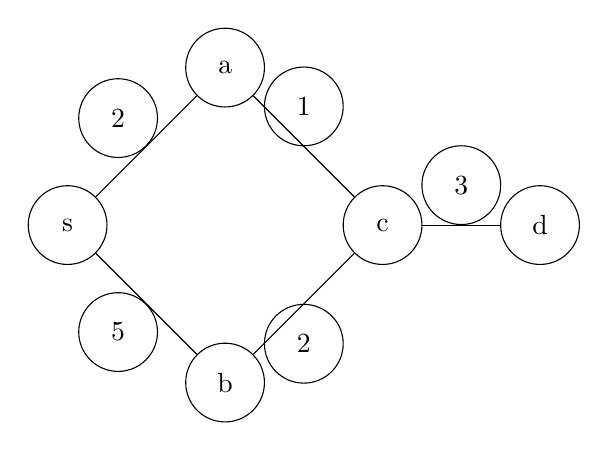
\begin{tikzpicture}[scale=1, every node/.style={circle, draw, minimum size=1cm}]
    % Nodes
    \node (s) at (0, 0) {s};
    \node (a) at (2, 2) {a};
    \node (b) at (2, -2) {b};
    \node (c) at (4, 0) {c};
    \node (d) at (6, 0) {d};
    
    % Edges with weights
    \draw (s) -- node[above left] {2} (a);
    \draw (s) -- node[below left] {5} (b);
    \draw (a) -- node[above] {1} (c);
    \draw (b) -- node[below] {2} (c);
    \draw (c) -- node[above] {3} (d);
\end{tikzpicture}
\end{center}

\begin{itemize}
    \item[\( \rhd \)] \textbf{Initialisation} :
    \begin{itemize}
        \item[\( \bullet \)] \( EM = \{ s \} \), \( \delta_s = 0 \), \( \delta_a = \delta_b = \delta_c = \delta_d = +\infty \).
    \end{itemize}
    \item[\( \rhd \)] \textbf{Itération 1} :
    \begin{itemize}
        \item[\( \bullet \)] Depuis \( s \), mise à jour :
        \[
        \delta_a = \min(\delta_a, \delta_s + \lambda_{sa}) = 0 + 2 = 2
        \]
        \[
        \delta_b = \min(\delta_b, \delta_s + \lambda_{sb}) = 0 + 5 = 5
        \]
        \item[\( \bullet \)] Sélection de \( a \) (étiquette minimale 2), \( EM = \{ s, a \} \).
    \end{itemize}
    \item[\( \rhd \)] \textbf{Itération 2} :
    \begin{itemize}
        \item[\( \bullet \)] Depuis \( a \), mise à jour :
        \[
        \delta_c = \min(\delta_c, \delta_a + \lambda_{ac}) = 2 + 1 = 3
        \]
        \item[\( \bullet \)] Sélection de \( c \) (étiquette minimale 3), \( EM = \{ s, a, c \} \).
    \end{itemize}
    \item[\( \rhd \)] \textbf{Itération 3} :
    \begin{itemize}
        \item[\( \bullet \)] Depuis \( c \), mise à jour :
        \[
        \delta_d = \min(\delta_d, \delta_c + \lambda_{cd}) = 3 + 3 = 6
        \]
        \item[\( \bullet \)] Depuis \( b \), aucune mise à jour (étiquette inchangée).
        \item[\( \bullet \)] Sélection de \( b \) (étiquette 5), \( EM = \{ s, a, c, b \} \).
    \end{itemize}
    \item[\( \rhd \)] \textbf{Itération 4} :
    \begin{itemize}
        \item[\( \bullet \)] Depuis \( b \), mise à jour potentielle de \( c \), mais \( \delta_c \) reste 3 (déjà plus petit).
        \item[\( \bullet \)] Sélection de \( d \) (étiquette 6), \( EM = \{ s, a, c, b, d \} \).
    \end{itemize}
    \item[\( \rhd \)] \textbf{Terminaison} : Tous les sommets sont marqués. Les étiquettes finales sont :
    \[
    \delta_s = 0, \quad \delta_a = 2, \quad \delta_b = 5, \quad \delta_c = 3, \quad \delta_d = 6
    \]
\end{itemize}

\subsection*{Complexité}

\begin{itemize}
    \item[\( \blacktriangleright \)] L'algorithme de Dijkstra a une complexité en \( \mathcal{O}( |E| + |V| \log |V| ) \) lorsqu'il est implémenté avec une file de priorité (tas binaire).
\end{itemize}
\end{multicols*}


\end{document}

